\begin{practice}
    \subsection{Luyện tập}

    \begin{questions}[series=SBT]
        \item Thay dấu “?” bằng giá trị thích hợp và hoàn thành bảng sau vào vở:

        \begin{center}
            \begin{tblr}{
                colspec={Q[c,m,2.2cm] Q[c,m,2cm] Q[c,m,2cm] Q[c,m,2.7cm] Q[c,m,2.2cm]},
                cells={valign=m},
                row{1}={font=\bfseries}
            }
                Hình & Bán kính đáy (cm) & Chiều cao (cm) & Diện tích xung quanh (cm$^2$) & Thể tích (cm$^3$) \\
                \SetCell[r=3]{c}
                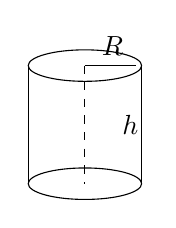
\begin{tikzpicture}
                    \coordinate (T) at (0,1.5);
                    \coordinate (B) at (0,0);
                    \draw (T) ellipse[x radius=.72,y radius=.2];
                    \draw (B) ellipse[x radius=.72,y radius=.2];
                    \draw (-.72,1.5)--(-.72,0) (.72,1.5)--(.72,0);
                    \draw[dashed] (T)--(B);
                    \draw (T)--(.65,1.5);
                    \node[right] at (.35,.75) {$h$};
                    \node[above] at (.35,1.5) {$R$};
                \end{tikzpicture}
                & 5 & 4 & ? & ? \\
                & 6 & ? & $96\pi$ & ? \\
                & ? & 10 & ? & $160\pi$
            \end{tblr}
        \end{center}

        \answerline
        \answerline

        \item Thay dấu “?” bằng giá trị thích hợp và hoàn thành bảng sau vào vở:

        \begin{center}
            \begin{tblr}{
                colspec={Q[c,m,2.3cm] Q[c,m,1.7cm] Q[c,m,1.7cm] Q[c,m,1.9cm] Q[c,m,2.35cm] Q[c,m,1.9cm]},
                cells={valign=m},
                row{1}={font=\bfseries}
            }
                Hình & Bán kính đáy (cm) & Chiều cao (cm) & Độ dài đường sinh (cm) & Diện tích xung quanh (cm$^2$) & Thể tích (cm$^3$) \\
                \SetCell[r=2]{c}
                \begin{tikzpicture}
                    \coordinate (O) at (0,0);
                    \coordinate (S) at (0,2);
                    \coordinate (A) at (-.85,0);
                    \coordinate (B) at (.85,0);
                    \draw (A) arc[start angle=180,end angle=360,x radius=.85,y radius=.22];
                    \draw[dashed] (B) arc[start angle=0,end angle=180,x radius=.85,y radius=.22];
                    \draw (S)--(A) (S)--(B);
                    \draw[dashed] (S)--(O);
                    \draw (O)--(B);
                    \node[right] at ($(S)!0.45!(O)$) {$h$};
                    \node[below] at ($(O)!0.5!(B)$) {$R$};
                    \node[right] at ($(S)!0.55!(B)$) {$l$};
                \end{tikzpicture}
                & 6 & 8 & ? & ? & ? \\
                & ? & ? & 13 & $65\pi$ & ?
            \end{tblr}
        \end{center}

        \answerline
        \answerline

        \item Bác Thu có một khối gỗ dạng hình trụ, chiều cao bằng $30$ cm, đường kính đáy bằng $20$ cm. Bác dự định sơn kín mặt ngoài của khối gỗ. Tính diện tích phần cần sơn (làm tròn kết quả đến hàng phần mười của cm$^2$).

        \answerline
        \answerline
        \answerline

        \item Bạn Trang làm một chiếc mũ sinh nhật bằng giấy bìa màu, đường kính đáy bằng $16$ cm, độ dài đường sinh bằng $17$ cm. Tính diện tích bìa màu bạn Trang cần dùng để làm chiếc mũ sinh nhật đó (coi mép dán không đáng kể, làm tròn kết quả đến hàng đơn vị của cm$^2$).

        \answerline
        \answerline
        \answerline

        \item Một trục lăn sơn có dạng hình trụ, đường kính của đường tròn đáy bằng $5$ cm, chiều dài bằng $23$ cm (H.10.2). Sau khi lăn trọn vẹn liên tục $15$ vòng thì diện tích phần sơn được trên mặt tường phẳng là bao nhiêu?

        \begin{center}
            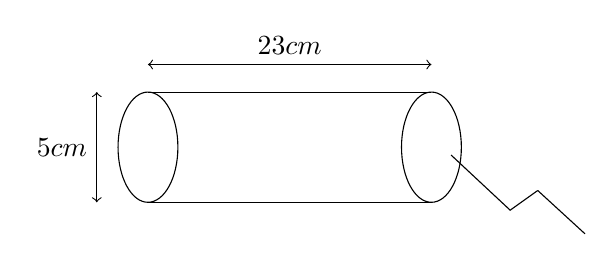
\begin{tikzpicture}
                \coordinate (L) at (0,0);
                \coordinate (R) at (3.6,0);
                \draw (L) ellipse[x radius=.38,y radius=.7];
                \draw (R) ellipse[x radius=.38,y radius=.7];
                \draw (0,.7)--(3.6,.7) (0,-.7)--(3.6,-.7);
                \draw[<->] (0,1.05)--(3.6,1.05) node[midway,above] {$23\text{ cm}$};
                \draw[<->] (-.65,-.7)--(-.65,.7) node[midway,left] {$5\text{ cm}$};
                \draw (3.85,-.1)--(4.6,-.8)--(4.95,-.55);
                \draw (4.95,-.55)--(5.55,-1.1);
            \end{tikzpicture}

            \textit{Hình 10.2}
        \end{center}

        \answerline
        \answerline
        \answerline

        \item Một công ty sản xuất vỏ lon nước ngọt bằng nhôm có dạng hình trụ kín hai đáy với đường kính đáy bằng $6{,}4$ cm và chiều cao bằng $12$ cm. Chi phí để sản xuất vỏ lon là khoảng $100\,000$ đồng/m$^2$. Hỏi số tiền công ty đó phải chi để sản xuất $2\,000$ vỏ lon nước ngọt là bao nhiêu (làm tròn kết quả đến hàng nghìn của cm$^2$)?

        \answerline
        \answerline
        \answerline
        \answerline

        \item Bác Khôi làm một dụng cụ bằng tôn gồm một phần có dạng hình trụ và một phần có dạng hình nón với các kích thước như Hình 10.3. Tính thể tích của dụng cụ này (coi mép hàn không đáng kể và làm tròn kết quả đến hàng đơn vị của cm$^3$).

        \begin{center}
            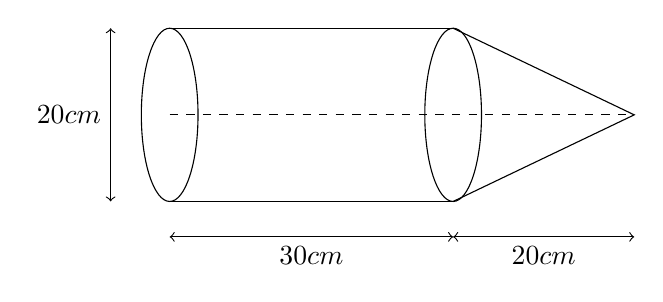
\begin{tikzpicture}
                \coordinate (L) at (0,0);
                \coordinate (R) at (3.6,0);
                \coordinate (S) at (5.9,0);
                \draw (L) ellipse[x radius=.36,y radius=1.1];
                \draw (R) ellipse[x radius=.36,y radius=1.1];
                \draw (0,1.1)--(3.6,1.1) (0,-1.1)--(3.6,-1.1);
                \draw (3.6,1.1)--(S)--(3.6,-1.1);
                \draw[dashed] (L)--(S);
                \draw[<->] (-.75,-1.1)--(-.75,1.1) node[midway,left] {$20\text{ cm}$};
                \draw[<->] (0,-1.55)--(3.6,-1.55) node[midway,below] {$30\text{ cm}$};
                \draw[<->] (3.6,-1.55)--(5.9,-1.55) node[midway,below] {$20\text{ cm}$};
            \end{tikzpicture}

            \textit{Hình 10.3}
        \end{center}

        \answerline
        \answerline
        \answerline
        \answerline
    \end{questions}
\end{practice}
